\documentclass[english,xcolor=svgnames]{beamer}


\usepackage{mathptmx}
\usepackage[OT1]{fontenc}
% \usepackage[latin9]{inputenc}
\usepackage{amsmath}
\usepackage{amssymb}
\usepackage{amsthm}
\usepackage{mathrsfs}
\usepackage{amsfonts}
\usepackage{eurosym}
\usepackage{bm}

\usepackage{booktabs}
\usepackage{tabularx}
\usepackage{subcaption}
\usepackage[makeroom,thicklines]{cancel}

\usepackage{multirow}
\usepackage{rotating}
\usepackage{array}
\usepackage{float}



\makeatletter

 \newcommand\makebeamertitle{\frame{\maketitle}}%
 \AtBeginDocument{
   \let\origtableofcontents=\tableofcontents
 \def\tableofcontents{\@ifnextchar[{\origtableofcontents}{\gobbletableofcontents}}
   \def\gobbletableofcontents#1{\origtableofcontents}
 }
 
 \usetheme{Boadilla}
\setbeamertemplate{footline}[frame number]{}
\usefonttheme{structuresmallcapsserif}
\setbeamercolor{title}{fg=blue}
\setbeamercolor{frametitle}{fg=blue}
\setbeamercolor{caption name}{fg=blue}
\setbeamercovered{transparent}


\beamertemplatenavigationsymbolsempty

\usepackage{booktabs}
\usepackage{tabularx}
\renewcommand{\tabularxcolumn}[1]{>{\centering\arraybackslash}m{#1}}
%\newcolumntype{L}{>{\centering}X}
%\newcolumntype{H}{>{\lrbox0}c<{\endlrbox}@{}}

%\let\estinput=\input
%\newcommand{\estwide}[3]{
%          \vspace{.75ex}{
%               \begin{tabularx}
%               {\textwidth}{@{\hskip\tabcolsep\extracolsep\fill}l*{#2}{#3}}
%               \toprule
%               \estinput{#1}
%               \bottomrule
%               \addlinespace[.75ex]
%               \end{tabularx}
%               }
%          }
%
%		\newcommand{\figtext}[1]{
%		     %\vspace{-1.9ex}
%		     \captionsetup{justification=justified,font=footnotesize}
%		     \caption*{\hspace{6pt}\hangindent=1.5em #1}
%		     }
%		\newcommand{\fignote}[1]{\figtext{\emph{Note:~}~#1}}
%
\usepackage{collcell}
%\makeatother
% \newcolumntype{G}{>{\collectcell\@gobble}c<{\endcollectcell}@{}}
% \makeatother
% \def\eatcell#1\unskip{}
% \newcolumntype{E}{>{\eatcell}c@{}}
%\usepackage{tabulary}
%\usepackage{multirow}
%\usepackage{dcolumn}
%\usepackage{pdflscape}
%\usepackage{pdfpages}
% \usepackage{epsfig}
% \usepackage{epstopdf}
% \usepackage{eso-pic}
\usepackage{graphicx}
%\usepackage{arydshln}
\usepackage[compatibility=false,font={sc,rm,color=blue},justification=centering,labelformat=empty, textfont=Large, margin=2pt]{caption}
\captionsetup[figure]{belowskip=0pt}

\newcommand{\rot}[2]{\rule{1em}{0pt}%
\makebox[0cm][c]{\rotatebox{#1}{\ #2}}}

\usepackage{siunitx} %For aligning decimals
\sisetup{ detect-mode, 
          group-digits            = false ,
          input-signs             = ,
          input-symbols           = ()[]-+* ,
          input-open-uncertainty  = ,
          input-close-uncertainty = ,
          table-align-text-post   = false, 
          table-number-alignment = center
}
\selectcolormodel{cmyk}
\usepackage{color,soul}
\usepackage{colortbl}
\usepackage{tikz}
\usetikzlibrary{matrix,shapes,arrows,intersections,calc}
\usepackage{verbatim}
\setbeamercovered{invisible}
\setbeamercolor{math text displayed}{fg=blue}
\setbeamercolor{math text inlined}{fg=blue}

%\let\olditem\item
%\renewcommand{\item}{\setlength{\itemsep}{\fill}\olditem}
\AtBeginDocument{\setlength\belowdisplayskip{0pt}}


\usepackage[english]{babel}
\usepackage{booktabs}
\usepackage{tablefootnote}
\usepackage{calc,hhline,ifthen,lscape} 

%\usepackage{enumitem}
%\let\olditem\item
%\renewcommand{\item}{\setlength{\itemsep}{\fill}\olditem}

% new math commands
\newcommand{\E}{\mathbb{E}}

\newcommand{\sym}[1]{\rlap{$#1$}} %For sym in STATA tables

\setbeamertemplate{frametitle}[default][center]

% \makeglossaries
% 
% \usepackage{pgfpages}
% \pgfpagesuselayout{resize to}[a4paper, landscape, border shrink=5mm]
\usepackage[absolute,overlay]{textpos}

\usepackage{epstopdf}


%\setlength{\itemsep}{\fill}



% ===========================================================
% ===========================================================
% ===========================================================
% Improves spacing of itemize and enumerate environment

\makeatletter
\renewcommand{\itemize}[1][]{%
  \beamer@ifempty{#1}{}{\def\beamer@defaultospec{#1}}%
  \ifnum \@itemdepth >2\relax\@toodeep\else
    \advance\@itemdepth\@ne
    \beamer@computepref\@itemdepth% sets \beameritemnestingprefix
    \usebeamerfont{itemize/enumerate \beameritemnestingprefix body}%
    \usebeamercolor[fg]{itemize/enumerate \beameritemnestingprefix body}%
    \usebeamertemplate{itemize/enumerate \beameritemnestingprefix body begin}%
    \list
      {\usebeamertemplate{itemize \beameritemnestingprefix item}}
      {\def\makelabel##1{%
          {%
            \hss\llap{{%
                \usebeamerfont*{itemize \beameritemnestingprefix item}%
                \usebeamercolor[fg]{itemize \beameritemnestingprefix item}##1}}%
          }%
        }%
      }
  \fi%
  \setlength\itemsep{\fill}
    \ifnum \@itemdepth >1
        \vfill
    \fi%  
  \beamer@cramped%
  \raggedright%
  \beamer@firstlineitemizeunskip%
}

\def\enditemize{\ifhmode\unskip\fi\endlist%
  \usebeamertemplate{itemize/enumerate \beameritemnestingprefix body end}
  \ifnum \@itemdepth >1
        \vfil
  \fi%  
  }
\makeatother


\makeatletter
\def\enumerate{%
	\ifnum\@enumdepth>2\relax\@toodeep
	\else%
	\advance\@enumdepth\@ne%
	\edef\@enumctr{enum\romannumeral\the\@enumdepth}%
	\advance\@itemdepth\@ne%
	\fi%
	\beamer@computepref\@enumdepth% sets \beameritemnestingprefix
	\edef\beamer@enumtempl{enumerate \beameritemnestingprefix item}%
	\@ifnextchar[{\beamer@@enum@}{\beamer@enum@}}
\def\beamer@@enum@[{\@ifnextchar<{\beamer@enumdefault[}{\beamer@@@enum@[}}
\def\beamer@enumdefault[#1]{\def\beamer@defaultospec{#1}%
	\@ifnextchar[{\beamer@@@enum@}{\beamer@enum@}}
\def\beamer@@@enum@[#1]{% partly copied from enumerate.sty
	\@enLab{}\let\@enThe\@enQmark
	\@enloop#1\@enum@
	\ifx\@enThe\@enQmark\@warning{The counter will not be printed.%
		^^J\space\@spaces\@spaces\@spaces The label is: \the\@enLab}\fi
	\def\insertenumlabel{\the\@enLab}
	\def\beamer@enumtempl{enumerate mini template}%
	\expandafter\let\csname the\@enumctr\endcsname\@enThe
	\csname c@\@enumctr\endcsname7
	\expandafter\settowidth
	\csname leftmargin\romannumeral\@enumdepth\endcsname
	{\the\@enLab\hspace{\labelsep}}%
	\beamer@enum@}
\def\beamer@enum@{%
	\beamer@computepref\@itemdepth% sets \beameritemnestingprefix
	\usebeamerfont{itemize/enumerate \beameritemnestingprefix body}%
	\usebeamercolor[fg]{itemize/enumerate \beameritemnestingprefix body}%
	\usebeamertemplate{itemize/enumerate \beameritemnestingprefix body begin}%
	\expandafter
	\list
	{\usebeamertemplate{\beamer@enumtempl}}
	{\usecounter\@enumctr%
		\def\makelabel##1{{\hss\llap{{%
						\usebeamerfont*{enumerate \beameritemnestingprefix item}%
						\usebeamercolor[fg]{enumerate \beameritemnestingprefix item}##1}}}}}%
	\setlength\itemsep{\fill}
	\ifnum \@itemdepth >1
	\vfill
	\fi%  
	\beamer@cramped%
	\raggedright%
	\beamer@firstlineitemizeunskip%
}
\def\endenumerate{\ifhmode\unskip\fi\endlist%
	\usebeamertemplate{itemize/enumerate \beameritemnestingprefix body end}
	\ifnum \@itemdepth >1
	\vfil
	\fi%  
}
\makeatother

% ===========================================================
% ===========================================================
% ===========================================================


%\usepackage[colorlinks=true]{hyperref}

\hypersetup{colorlinks = true,linkcolor = blue, bookmarksopen=true, bookmarksopenlevel=1}

%\hypersetup{bookmarksopen=true, bookmarksopenlevel=1}



\begin{document}

\title{Household Aggregation}
\vspace{1cm}
\author[shortname]{
\begin{tabular}{cc}
Juan Herre\~{n}o & Johannes Wieland \\ 
\end{tabular}\\
}



\date{UCSD, Spring \the\year}

\setbeamertemplate{footline}{}
\makebeamertitle
\setbeamertemplate{footline}[frame number]{}

\addtocounter{framenumber}{-1}



\begin{frame}
\frametitle[alignment=center]{Reminders}
\begin{enumerate}
	\item First project draft due May 4.
	% \item Participation.
\end{enumerate}
\end{frame}


%%%%%%%%%%%%%%%%%%%%%%%%%%%%%%%%%%%%%%%%%%%%%%%%%%
\AtBeginSection[]{
\setbeamertemplate{footline}{}
  \frame<beamer>{ 

    \frametitle{Outline}   

    \tableofcontents[currentsection,hideallsubsections] 
  }
\setbeamertemplate{footline}[frame number]{}
\addtocounter{framenumber}{-1}
}

\AtBeginSubsection[]{
\setbeamertemplate{footline}{}
  \frame<beamer>{ 

    \frametitle{Outline}   

    \tableofcontents[currentsection,currentsubsection] 
  }
  \setbeamertemplate{footline}[frame number]{}
  \addtocounter{framenumber}{-1}
}



\setbeamertemplate{footline}{}
\begin{frame}
\frametitle{Outline}   
\tableofcontents[hideallsubsections] 
\end{frame}
\addtocounter{framenumber}{-1}
\setbeamertemplate{footline}[frame number]{}




%%%%%%%%%%%%%%%%%%%%%%%%%%%%%%%%%%%%%%%%%%%%%%%%%%
\section{Parker, Souleles, Johnson, and McClelland (2013, AER)}
%%%%%%%%%%%%%%%%%%%%%%%%%%%%%%%%%%%%%%%%%%%%%%%%%%

\begin{frame}
\frametitle[alignment=center]{What is the MPC?}
\begin{itemize}
	\item MPC = marginal propensity to consume.
	\item Very important parameter in old Keynesian models.
	\item In standard New Keynesian models $\approx 0$.
	\begin{itemize}
		\item Euler equation $\Rightarrow$ Permanent income consumer.
	\end{itemize}
	\item TANK and HANK models.
\end{itemize}
\end{frame}

\begin{frame}
\frametitle[alignment=center]{Identification Problem}
\begin{align*}
	c_{it}  = \alpha + \beta y_{it} + \epsilon_{it}
\end{align*}
\begin{itemize}
	\item What could go wrong?
\end{itemize}
\end{frame}

\begin{frame}
\frametitle[alignment=center]{Jonathan Parker Oeuvre}
\begin{itemize}
	\item Johnson, Parker, Souleles, AER 2003: 20-40\% of 2001 Rebate spent on nondurable goods within 3 months.
	\item Parker, Souleles, Johnson, McClelland, AER 2008: 50-90\% of 2008 Rebate spent on nondurable and durable goods within 3 months.
	\item Broda, Parker, JME 2014: 2008 rebate caused 10\% increase in spending in first week.
	\item Parker, Schild, Erhard, Johnson, WP 2022: 10\% of 2020 stimulus was spent within 3 months.
\end{itemize}
\end{frame}

\begin{frame}
\frametitle[alignment=center]{The 2008 Experiment}
\centering
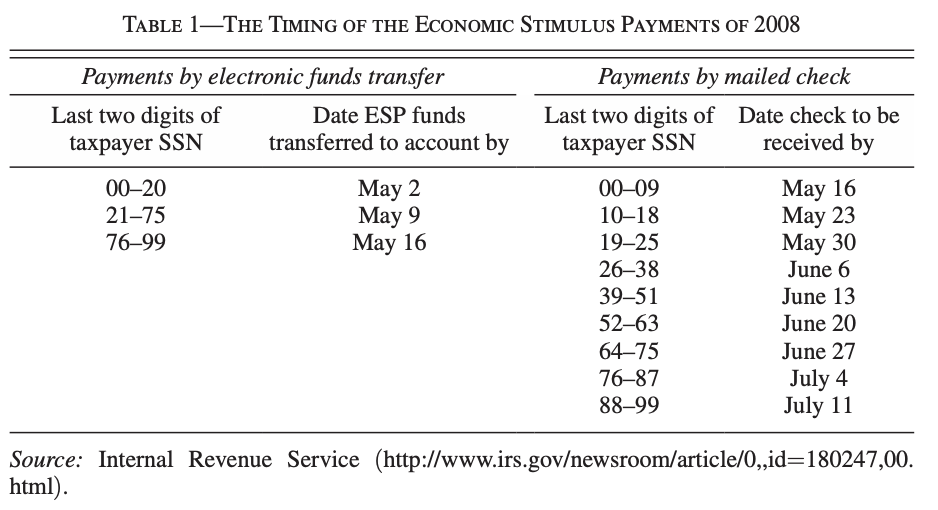
\includegraphics[scale=0.6]{figures/PSMJTAB1.png}
\end{frame}

\begin{frame}
\frametitle[alignment=center]{Specification}
\begin{align*}
	C_{i,t+1}-C_{i,t} = \sum_s \beta_{0s} \times month_{s,i} + \beta_1'X_{i,t} + \beta_2 ESP_{i,t+1} + u_{i,t+1}
\end{align*}
\begin{itemize}
	\item Comments? Concerns?
\end{itemize}
\end{frame}

\begin{frame}
\frametitle[alignment=center]{Effects on Expenditure}
\centering
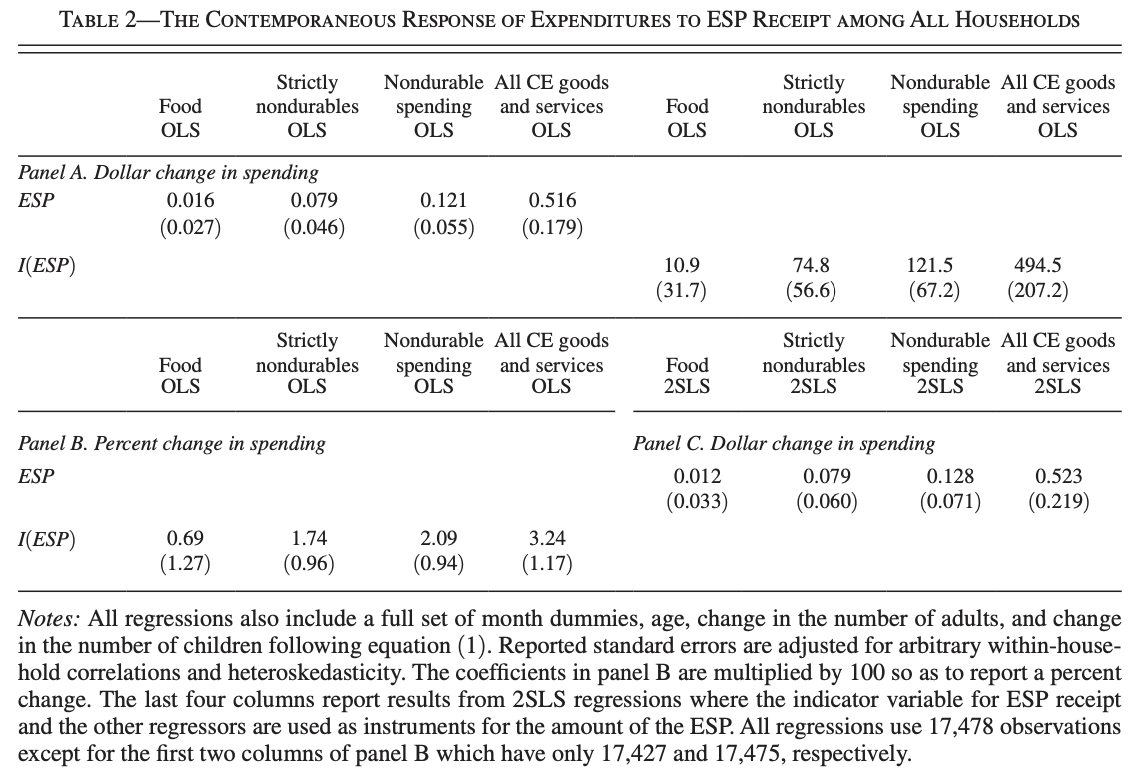
\includegraphics[scale=0.6]{figures/PSMJTAB2.png}
\end{frame}

\begin{frame}
\frametitle[alignment=center]{Sub-Samples}
\centering
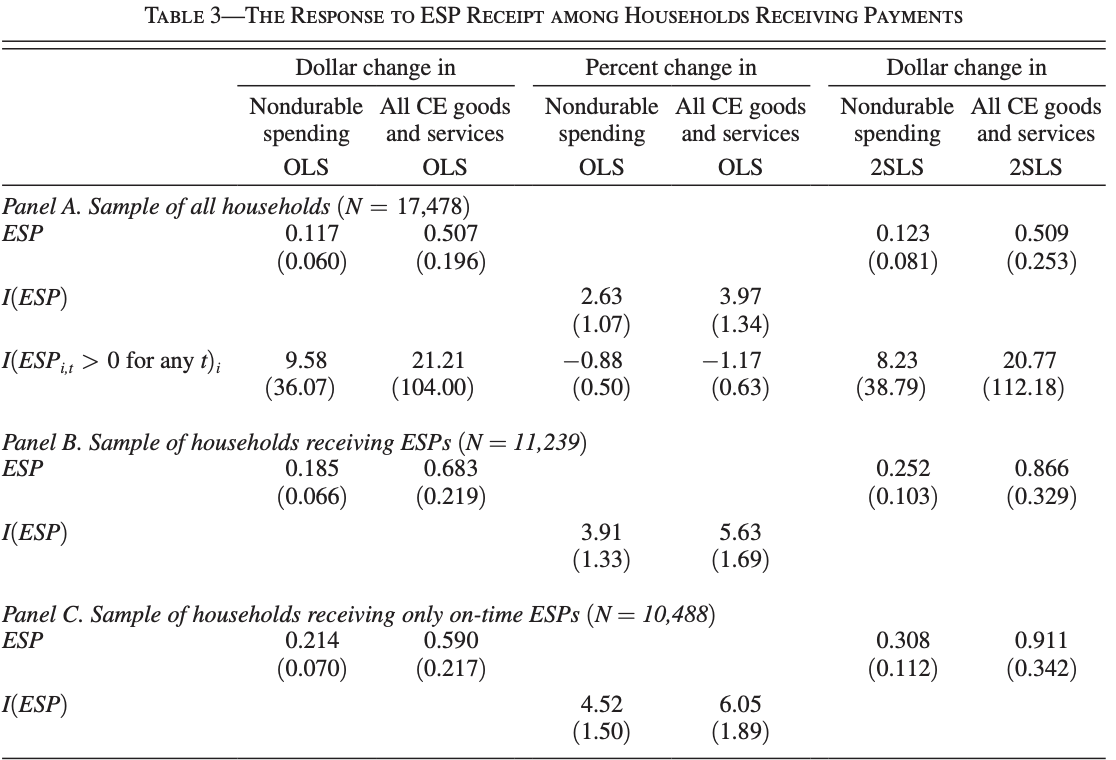
\includegraphics[scale=0.6]{figures/PSMJTAB3.png}
\end{frame}

\begin{frame}
\frametitle[alignment=center]{Persistence}
\centering
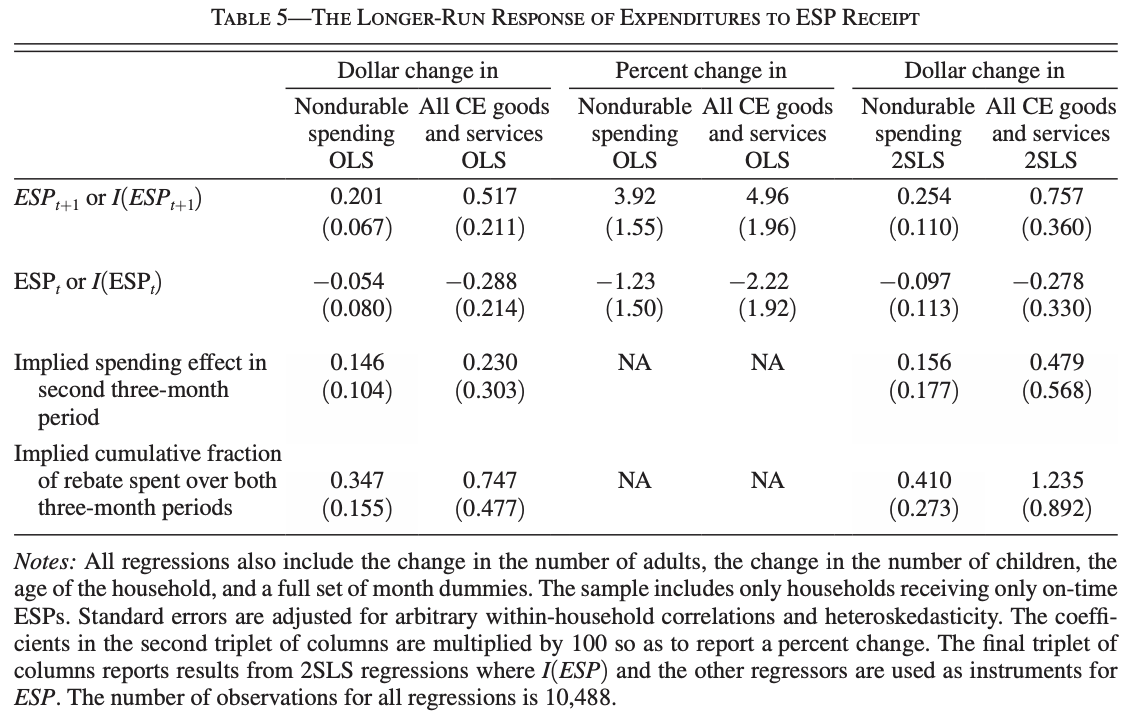
\includegraphics[scale=0.6]{figures/PSMJTAB5.png}
\end{frame}


\begin{frame}
\frametitle[alignment=center]{Heterogeneous Treatment Effects}
\centering
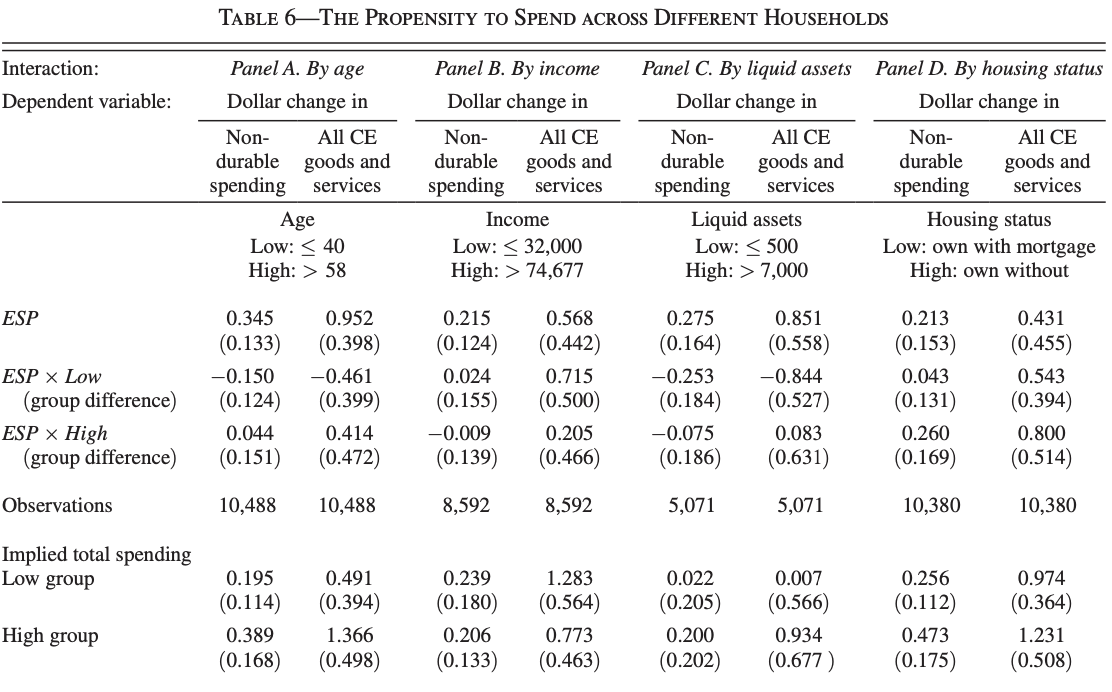
\includegraphics[scale=0.6]{figures/PSMJTAB6.png}
\end{frame}


\begin{frame}
\frametitle[alignment=center]{Convincing?}

\end{frame}

\begin{frame}
\frametitle[alignment=center]{More MPCs}
\begin{itemize}
	\item Shapiro and Slemrod (AER 2003, AER, 2009): self-reported MPC of 25-30\% out of rebates in 2001 / 2008.
	\item Japielli and Pistaferri (AEJ-Macro, 2014): self-reported MPC of 48\% out of hypothetical transitory income shock.
	\item Faegereng, Holmn, and Natvick (AEJ-Macro, 2021): 50\% MPC within one year of large lottery winnings in Norway. Consumption is resiaul from budget constraint: $C=Y - \Delta A$.
\end{itemize}
\end{frame}


%%%%%%%%%%%%%%%%%%%%%%%%%%%%%%%%%%%%%%%%%%%%%%%%%%
\section{de Chaisemartin and D'Haultf{\oe}uille (2020, AER)}
%%%%%%%%%%%%%%%%%%%%%%%%%%%%%%%%%%%%%%%%%%%%%%%%%%

\begin{frame}
\frametitle[alignment=center]{de Chaisemartin and D'Haultf{\oe}uille, AER 2020}
\begin{itemize}
	\item Panel, binned into cells $g,t$ (g=group).
	\item $Y_{i,g,t}$ outcome of unit $i$ in cell $g,t$.
	\item $D_{g,t}$ treatment indicator.
	\item Expectation of OLS 2-way FE estimator:
	\begin{align*}
		\beta_{fe} = E \left(\sum_{(g,t):D_{g,t}=1} W_{g,t}\Delta_{g,t}\right)
	\end{align*}
	\begin{itemize}
		\item $W_{g,t}$ are weights, $\sum_{(g,t):D_{g,t}=1} W_{g,t}=1$.
		\item $\Delta_{g,t}$ is the group-specific ATE.
	\end{itemize}
\end{itemize}
\end{frame}

\begin{frame}
\frametitle[alignment=center]{What is the Problem?}
\begin{itemize}
	\item With homogeneous treatment effects, no problem:
	\begin{align*}
		 \Delta_{g,t}=\Delta \;\Rightarrow\; \beta_{fe} = \Delta
	\end{align*}
	\item With heterogenous treatment effects $\beta_{fe}$ may be poor guide to average ATE since weights $W_{g,t}$ may be negative.
\end{itemize}
\end{frame}

%%%%%%%%%%%%%%%%%%%%%%%%%%%%%%%%%%%%%%%%%%%%%%%%%%
\section{Borusyak, Jaravel, and Spiess (2022, WP)}
%%%%%%%%%%%%%%%%%%%%%%%%%%%%%%%%%%%%%%%%%%%%%%%%%%

\begin{frame}
\frametitle[alignment=center]{Borusyak, Jaravel, and Spiess, WP 2022}
\begin{center}
	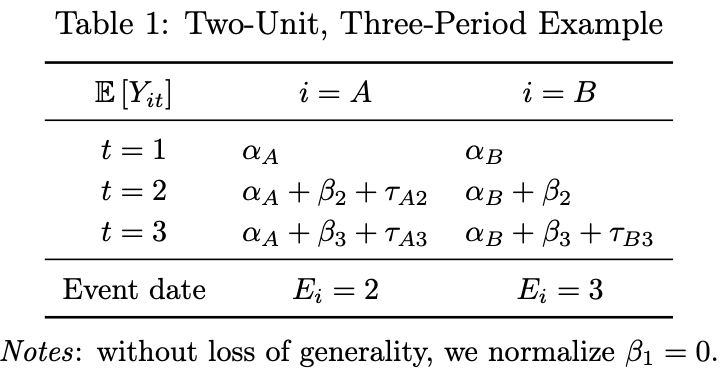
\includegraphics[scale=0.5]{figures/BJSTAB1.png}
\end{center}
\begin{itemize}
	\item 2-way FE OLS population coefficient is:
	\begin{align*}
		\beta_{fe} = \tau_{A2} + \frac{1}{2}\tau_{B3} - \frac{1}{2}\tau_{A3}
	\end{align*}
	\item Not an ATE!
	\item What is OLS doing here?
%	\item Do we get an ATE if we add a lag?
\end{itemize}
\end{frame}


\begin{frame}
\frametitle[alignment=center]{Test for Pre-Trends}
\begin{center}
	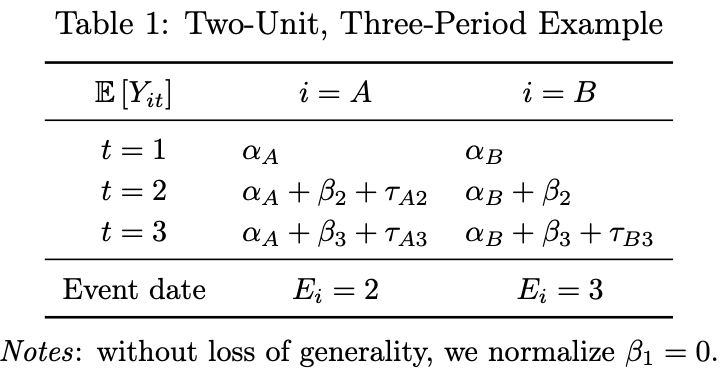
\includegraphics[scale=0.5]{figures/BJSTAB1.png}
\end{center}
\begin{itemize}
	\item Pre-trend coefficient for lag 2:
	\begin{align*}
		\beta_{fe,-2} &= \tau_{A3} - \tau_{B3}
	\end{align*}
	\item What is OLS doing here?
	\item Identified?
\end{itemize}
\end{frame}

\begin{frame}
\frametitle[alignment=center]{Notation}
\begin{itemize}
	\item Binary treatment $D_{it}$, outcome $Y_{it}$
	\item Event date $E_{it}$ where $D_{it}$ switches from 0 to 1.
	\item Observations $\Omega_1=\{it\in \Omega:\; D_{it}=1\}$ and not-yet-treated $\Omega_0$ (includes never treated). 
	\begin{itemize}
		\item Treated: $\Omega_1=\{it\in \Omega:\; D_{it}=1\}$, $|\Omega_1|=N_1$
		\item Not-yet-treated: $\Omega_0=\{it\in \Omega:\; D_{it}=0\}$, $|\Omega_0|=N_0$
	\end{itemize}
	\item $Y_{it}(0)$ potential outcome if never treated.
	\item Causal effect $\tau_{it}=E[Y_{it}-Y_{it}(0)]$.
\end{itemize}
\end{frame}

\begin{frame}
\frametitle[alignment=center]{Start from First Principles}
\begin{itemize}
	\item Estimation target:
	\begin{align*}
		\tau_w = \sum_{it\in\Omega_1} w_{it}\tau_{it} = w'\tau
	\end{align*}
	\item Assumption 1: Parallel trends 
	\begin{align*}
		E[Y_{it}(0)] = \alpha_i + \beta_t \qquad\forall it\in \Omega
	\end{align*}
	\item Assumption 2: No anticipation
	\begin{align*}
		Y_{it}=Y_{it}(0) \qquad\forall it\in \Omega_0
	\end{align*}
	\item Assumption 3': Restricted causal effects
	\begin{align*}
		\tau =\Gamma \theta 
	\end{align*}
	\begin{itemize}
		\item $\theta$ is unknown $N_1-M \times 1$, $\Gamma$ is known $N_1\times (N_1-M$)
		\item $M$ restrictions on treatment effect. $M=N_1-1$ = homogenous effects.
	\end{itemize}
\end{itemize}
\end{frame}

\begin{frame}
\frametitle[alignment=center]{BSJ Theorem 1 [Simplified]}
\begin{itemize}
	\item Suppose Assumptions 1, 2, 3', and 4 [homoscedastic errors] hold. Then among linear unbiased estimators of $\tau_w$, the (unique) efficient estimator $\hat{\tau}_w^*$ can be obtained with the following steps:
	\begin{enumerate}
		\item Estimate $\theta$ by $\hat{\theta}$ from the linear regression
		\begin{align*}
			Y_{it} = \alpha_i + \beta_t + D_{it}\Gamma_{it}'\theta + \epsilon_{it}.
		\end{align*}
		\item Estimate the vector of treatment effects $\tau$ by $\hat{\tau}=\Gamma \hat{\theta}$.
		\item Estimate the target $\tau_t$ by $\hat{\tau}_w^* = w'\hat{\tau}$
	\end{enumerate}
\end{itemize}
\end{frame}

\begin{frame}
\frametitle[alignment=center]{BSJ Theorem 2 [Simplified]}
\begin{itemize}
	\item With unrestricted treatment effects $(M=0$), the unique efficient linear unbiased estimator $\hat{\tau}_w^*$ of $\tau_w$ from Theorem 1 can be obtained via an imputation procedure:
	\begin{enumerate}
		\item Within the untreated observations only ($it\in \Omega_0$), estimate by OLS:
		\begin{align*}
			Y_{it} = \alpha_i + \beta_t + \epsilon_{it}.
		\end{align*}
		\item For each treated observations ($it\in \Omega_1$) with $w_{it}\neq 0$, set  $\hat{Y}_{it}(0) = \hat{\alpha}_i + \hat{\beta}_t$ and $\hat{\tau}_{it} = \hat{Y}_{it} - \hat{Y}_{it}(0)$.
		\item Estimate the target $\tau_w$ by a weighted sum $\hat{\tau}_w^*=w'\hat{\tau}$
	\end{enumerate}
\end{itemize}
\end{frame}


\begin{frame}
\frametitle[alignment=center]{Inference}
\begin{itemize}
	\item Inference problem for treated units:
	\begin{align*}
			Y_{it} = \alpha_i + \beta_t + \tau_{it} + \epsilon_{it}.
		\end{align*}
	\item How to distinguish between unrestricted $\tau_{it}$ and $\epsilon_{it}$?
	\item ``Conservative'' standard errors: impose some homogeneity, so attribute some variance to $\epsilon_{it}$ that belongs to $\tau_{it}$.
	\item Yields asymptotically weakly conservative standard errors.
\end{itemize}
\end{frame}

\begin{frame}
\frametitle[alignment=center]{Pre-trends}
\begin{itemize}
	\item To test for pre-trends augment model for untreated observations with additional pre-determined variables and test that the coefficients are zero.
	\item Does not distort inference conditional on test passing.
	\item What happens if we then include these variables in the regression model? Do we satisfy parallel trends?
\end{itemize}
\end{frame}


\begin{frame}
\frametitle[alignment=center]{Application to Broda and Parker, JME 2014}
\centering
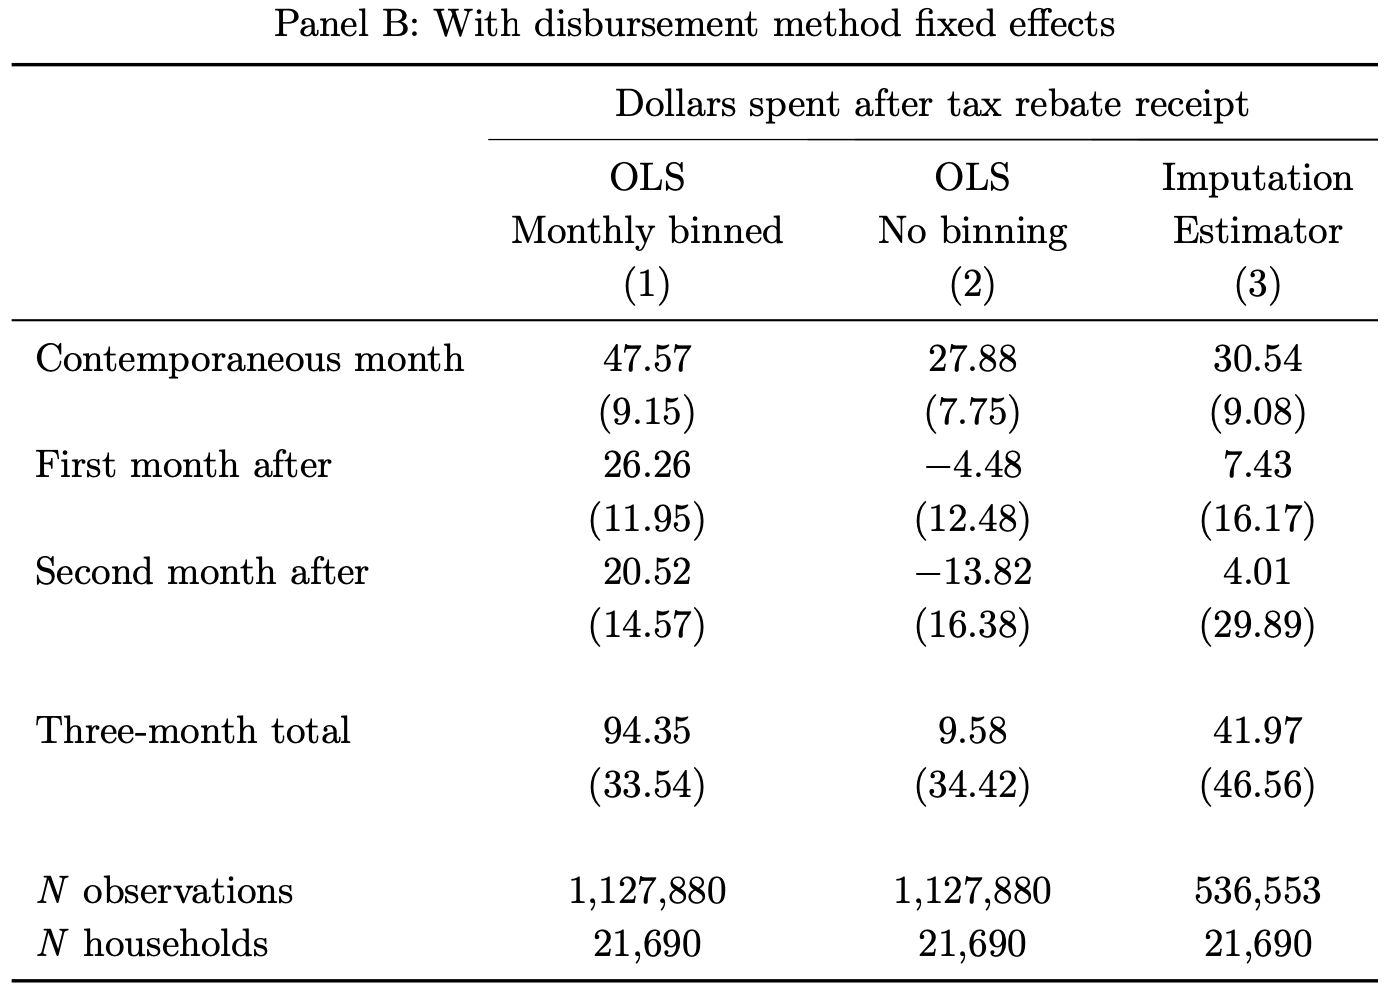
\includegraphics[scale=0.4]{figures/BJSTAB3a.png}
\end{frame}

\begin{frame}
\frametitle[alignment=center]{Dynamic Treatment Effects}
\centering
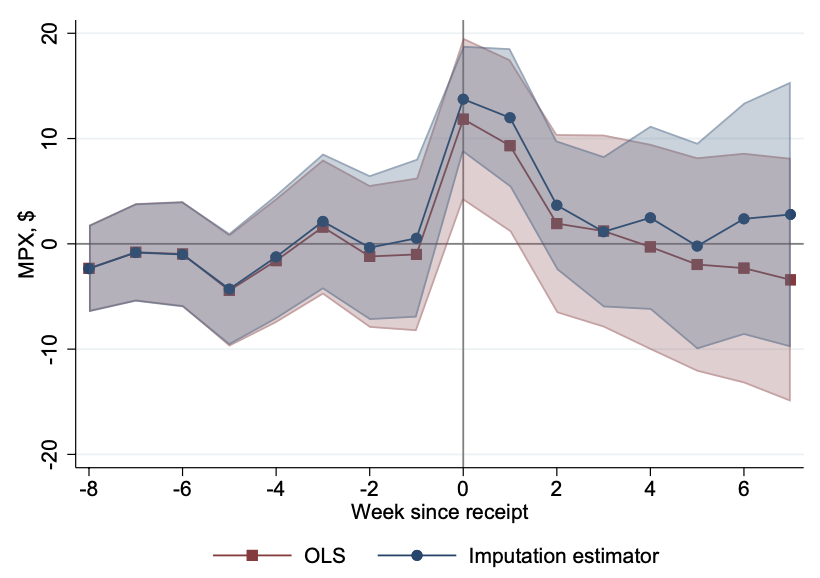
\includegraphics[scale=0.5]{figures/BJSFIG2b.png}
\end{frame}

\begin{frame}
\frametitle[alignment=center]{Weights}
\centering
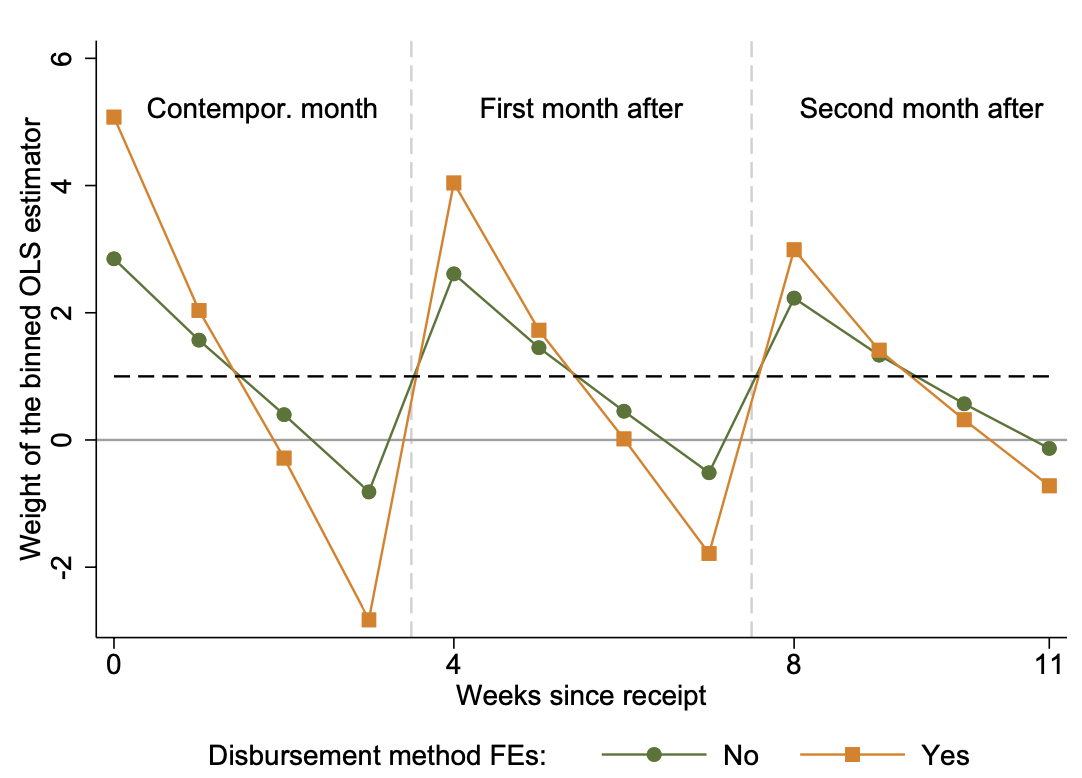
\includegraphics[scale=0.5]{figures/BJSFIG3.png}
\end{frame}

%%%%%%%%%%%%%%%%%%%%%%%%%%%%%%%%%%%%%%%%%%%%%%%%%%
\section{Orchard, Ramey, and Wieland (2022, WP)}
%%%%%%%%%%%%%%%%%%%%%%%%%%%%%%%%%%%%%%%%%%%%%%%%%%


\begin{frame}{}
\frametitle{Expenditures on New Motor Vehicles: Actual vs. Counterfactual}

\begin{center}
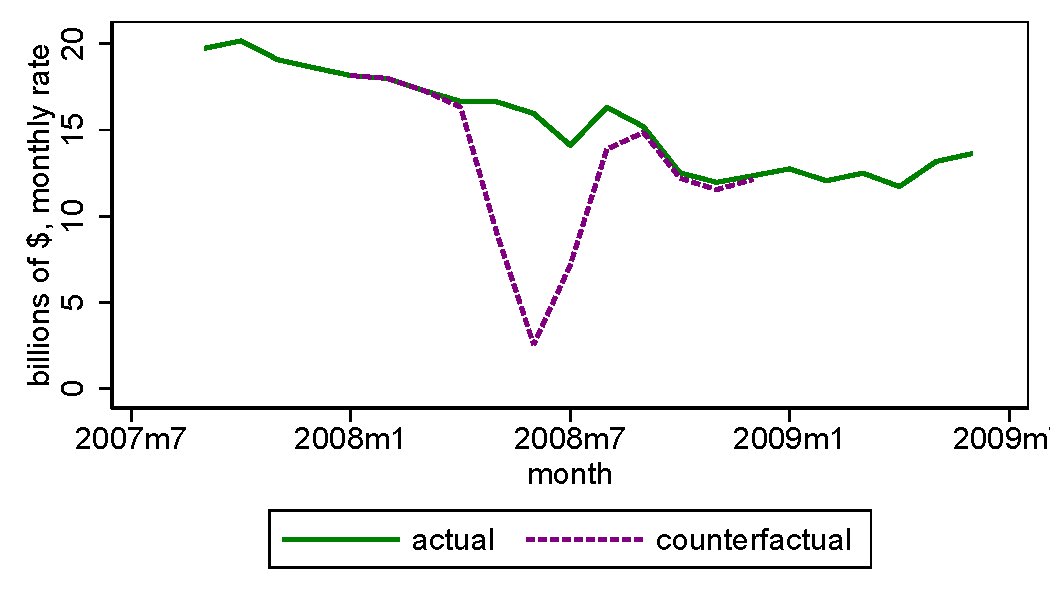
\includegraphics[scale=.6]{figures/fig_sss_mv_counter.pdf}
 \end{center} 
{\footnotesize Update of Sahm, Shapiro, Slemrod (2012) calculation, no general equilibrium feedbacks.}
\end{frame}

\begin{frame}
\frametitle[alignment=center]{G.E. Effects Can Increase Puzzle }
\begin{itemize}

	\item Direct micro effect - governed by \textit{micro MPC} .
\item Induced macro effect - governed by \textit{general equilibrium MPC} (\textcolor{red}{GE-MPC}) \hspace{.05in} \\ \vspace{.2in}
\indent GE-MPC \hspace{.05in} = \hspace{.05in} micro MPC \hspace{.05in} + \hspace{.05in} induced macro effect \hspace{.05in} \\ \medskip
\indent \hspace{0.62in}  $\equiv$ \hspace{.05in} \text{the multiplier in a closed economy with no capital}.


\end{itemize}



\end{frame}

\begin{frame}{Methodology for creating macro counterfactuals}
\vspace{.1in}

  \begin{itemize}\itemsep=4ex
  \item Construct a medium-scale \textcolor{blue}{two-good, two-agent} New Keynesian model with nondurables and durables (interpreted as motor vehicles).
  \item Calibrate fraction of \textcolor{blue}{hand-to-mouth households} to match micro MPCs.
  \item \textcolor{blue}{Simulate} response of consumption to rebates.
  \item Subtract simulated responses from actual consumption data  from 2008 to derive the \textcolor{blue}{counterfactual path} with no rebate.
  \end{itemize}
\end{frame}

\begin{frame}[label=baselineforecasts]
\frametitle{Counterfactual Consumption Expenditure: Baseline Model}

\begin{center}
\footnotesize
\centering
    \begin{tabular}{cc}
    Real PCE: Micro MPCs & Real PCE GE: Baseline \\
    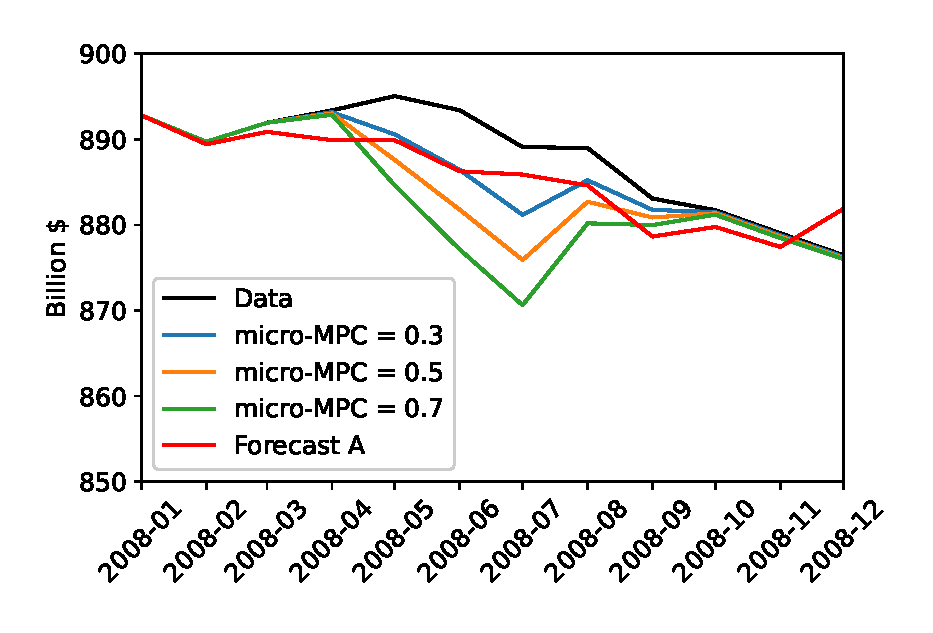
\includegraphics[width=5cm]{figures/Real_PCEfc_micro_baseline.eps} &   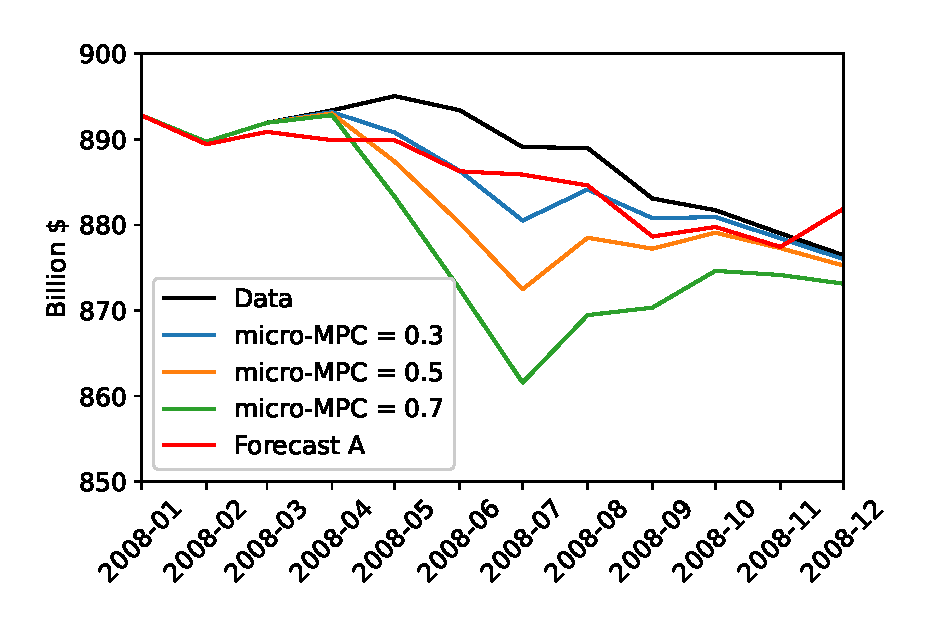
\includegraphics[width=5cm]{figures/Real_PCEfc_GE_baseline.eps} \\
    Motor Vehicles: Micro MPCs & Motor Vehicles: GE Baseline \\
    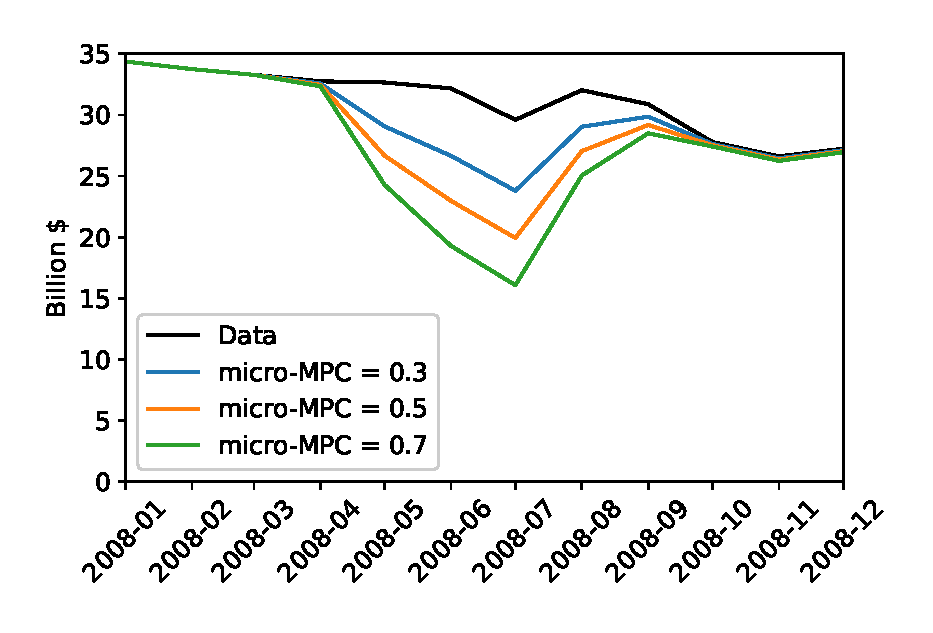
\includegraphics[width=5cm]{figures/Real_Motorvehicles_micro_baseline.eps} &  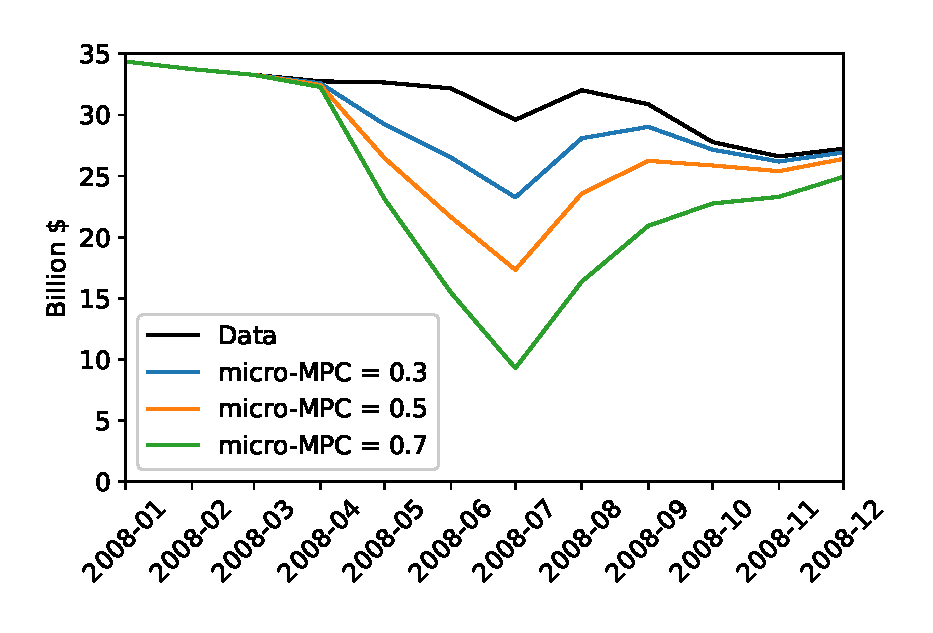
\includegraphics[width=5cm]{figures/Real_Motorvehicles_GE_baseline.eps} \\
    \end{tabular} \\
 \end{center} 
 \vspace{-0.5cm}
\end{frame}

\begin{frame}
\frametitle{Reconciling Implausible Macro G.E. Effects}

\begin{itemize}
	\item \textbf{G.E. Dampening}
		\begin{itemize}
		\item Key: 2/3 (or more) of estimated micro-mpc from new vehicle purchases
		\item Durable good demand is elastic and if supply is less elastic, G.E. effects can dampen micro-effects
		\end{itemize}
		
\item \textbf{Micro MPCs}
	\begin{itemize}
		\item Apply B.J.S. method to CEX data
		\item Resulting micro-mpc is .3 (compared to .52 in Parker et. al.)
		\item Why? Mostly explained by negative weights on past treated units
	\end{itemize}
\end{itemize}

\end{frame}

\begin{frame}{Decomposing OLS v.DID Imputation}
    \label{decompose_OLSd}

    \begin{figure}
    \centering
    \begin{tabular}{cc}
    Period Weights & Period Coefficients \\
    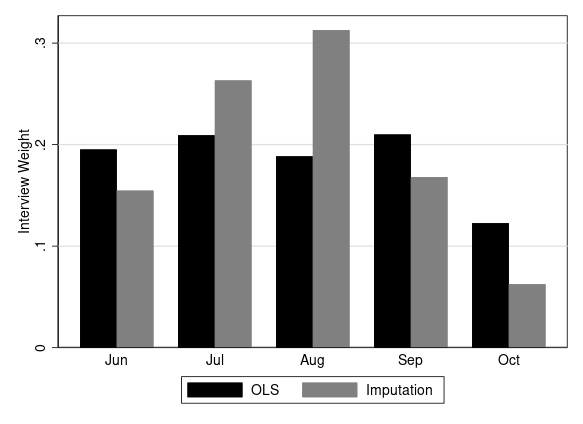
\includegraphics[width=4.5cm]{figures/BJSvOLSweight_d_totexp2_v2__} &   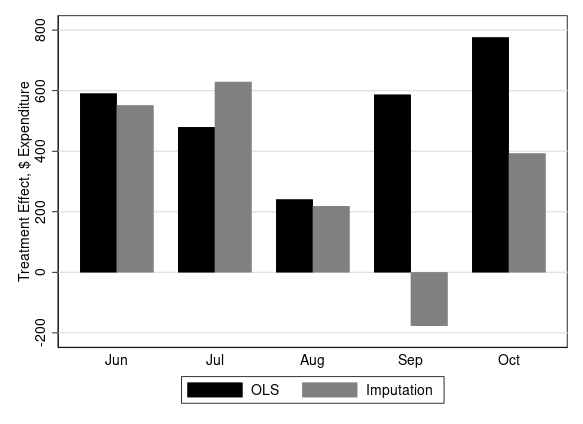
\includegraphics[width=4.5cm]{figures/BJSvOLScoef_d_totexp2_v2__} \\
    Decomposed Coefficient & Relative Contributions \\
   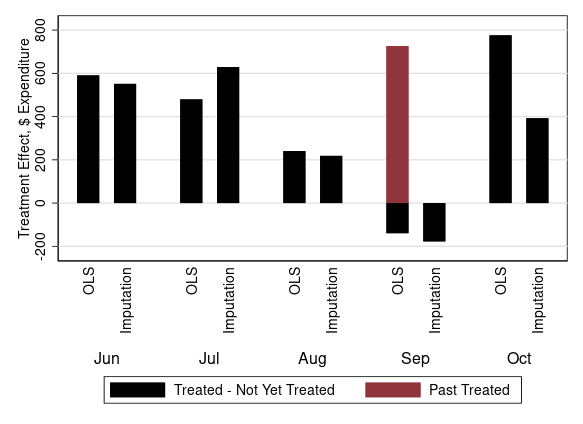
\includegraphics[width=4.5cm]{figures/BJSvOLScoef_stack_d_totexp2_v2__}& 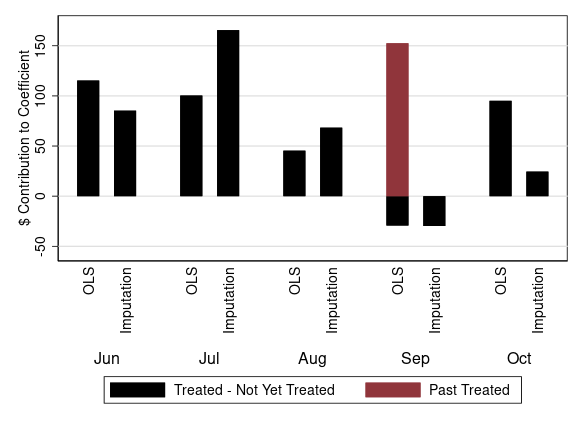
\includegraphics[width=4.5cm]{figures/BJSvOLScontribution_d_totexp2_v2__} \\
    \end{tabular} \\
    
\end{figure}
\end{frame}

\begin{frame}[label=durablepriceforecasts]
\frametitle{Counterfactual: Less Elastic Durable Supply Model}

\begin{center}
\footnotesize
\centering
    \begin{tabular}{cc}
    Real PCE: Micro MPCs & Real PCE: GE Less Elastic \\
    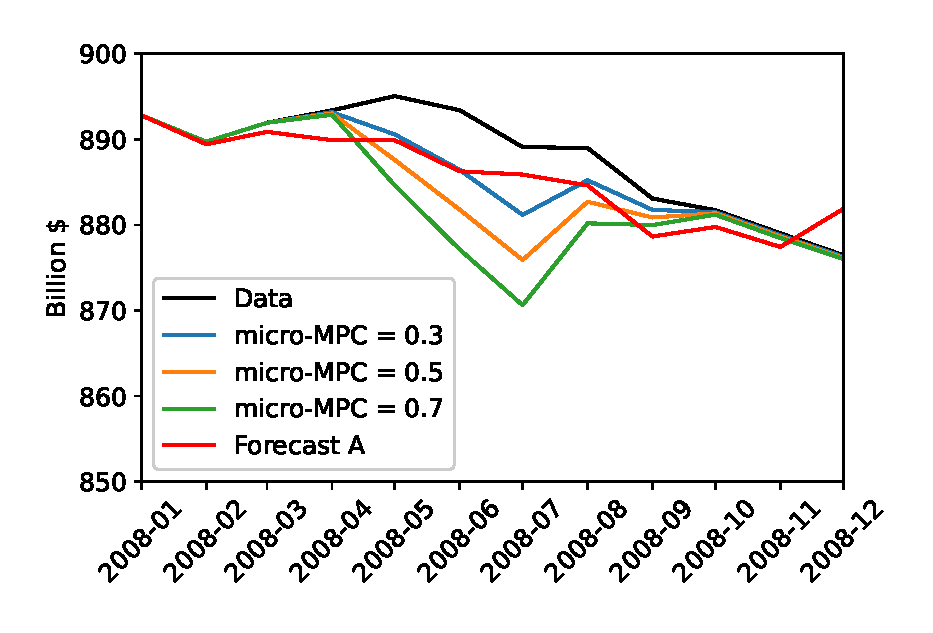
\includegraphics[width=5cm]{figures/Real_PCEfc_micro_durableprice.eps} &   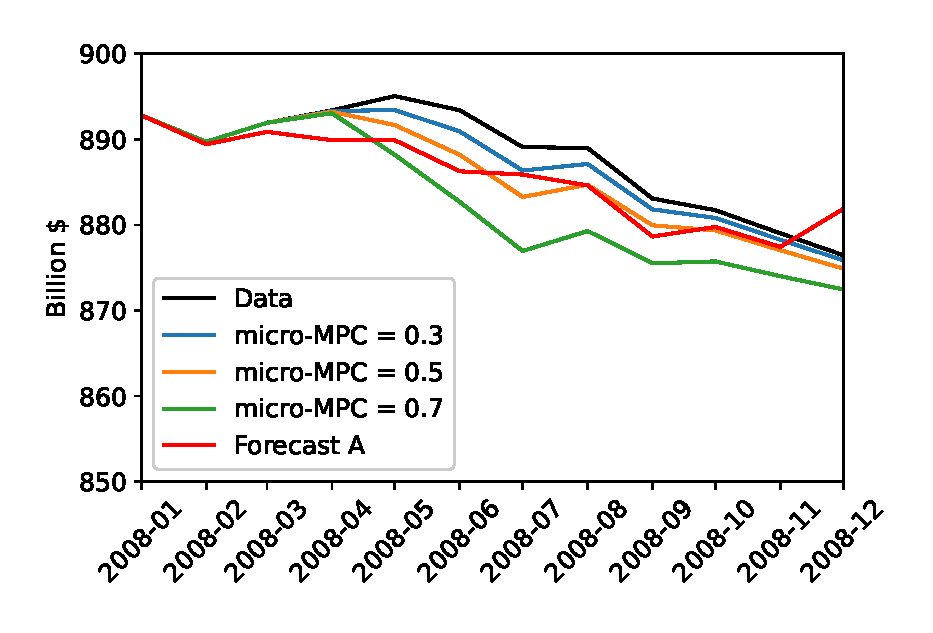
\includegraphics[width=5cm]{figures/Real_PCEfc_GE_durableprice.eps} \\
    Motor Vehicles: Micro MPCs & Motor Vehicles: GE Less Elastic \\
    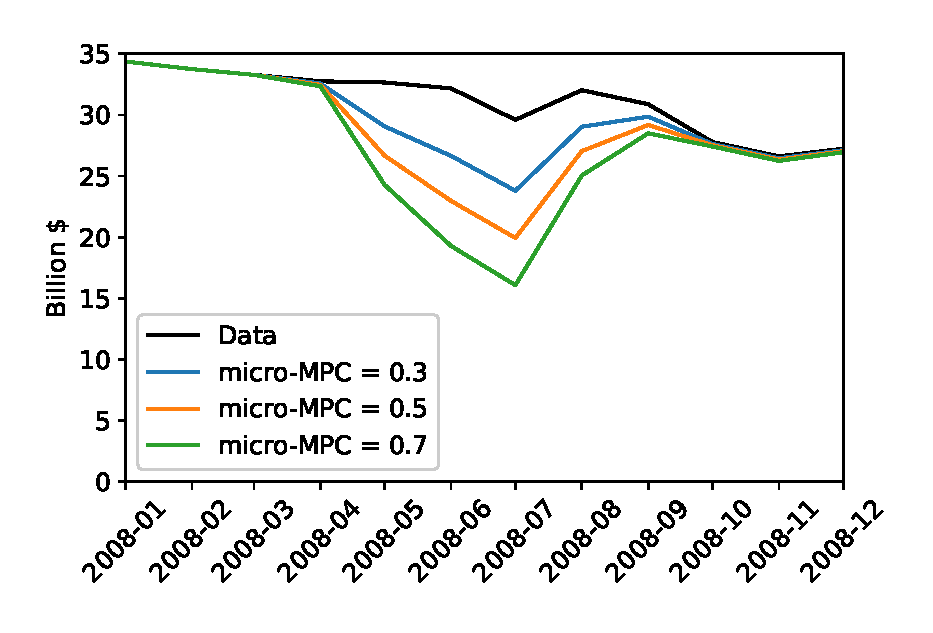
\includegraphics[width=5cm]{figures/Real_Motorvehicles_micro_durableprice.eps} &  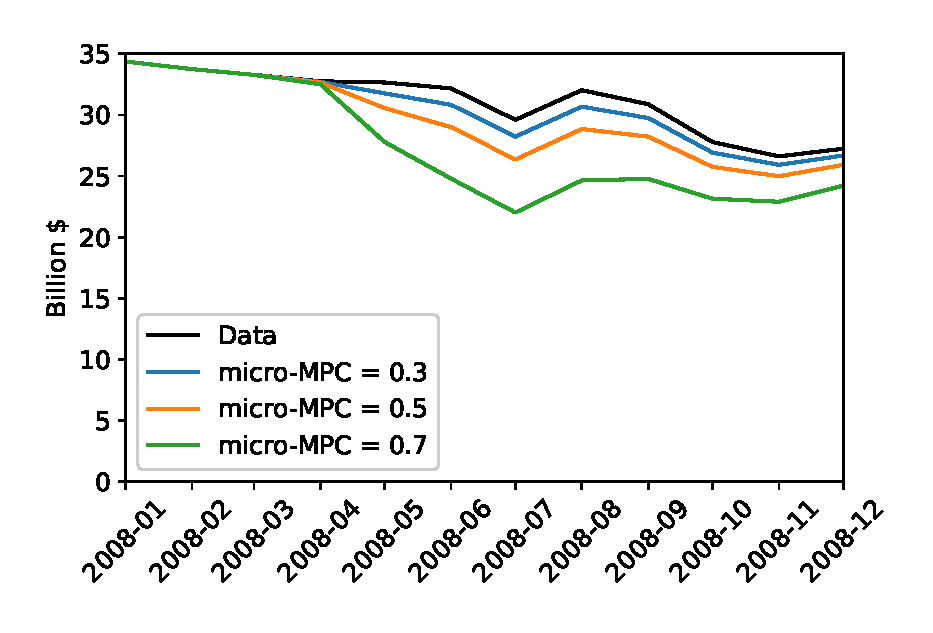
\includegraphics[width=5cm]{figures/Real_Motorvehicles_GE_durableprice.eps} \\
    \end{tabular} \\
 \end{center} 
 \vspace{-0.5cm}
\end{frame}

\end{document}